%
% This is a borrowed LaTeX template file for lecture notes for CS267,
% Applications of Parallel Computing, UCBerkeley EECS Department.
%

\documentclass[twoside]{article}
\setlength{\oddsidemargin}{0.25 in}
\setlength{\evensidemargin}{-0.25 in}
\setlength{\topmargin}{-0.6 in}
\setlength{\textwidth}{6.5 in}
\setlength{\textheight}{8.5 in}
\setlength{\headsep}{0.75 in}
\setlength{\parindent}{0 in}
\setlength{\parskip}{0.1 in}

%
% ADD PACKAGES here:
%

\usepackage{amsmath,amsfonts,graphicx}

%
% The following commands set up the lecnum (lecture number)
% counter and make various numbering schemes work relative
% to the lecture number.
%
\newcounter{lecnum}
\renewcommand{\thepage}{\thelecnum-\arabic{page}}
\renewcommand{\thesection}{\thelecnum.\arabic{section}}
\renewcommand{\theequation}{\thelecnum.\arabic{equation}}
\renewcommand{\thefigure}{\thelecnum.\arabic{figure}}
\renewcommand{\thetable}{\thelecnum.\arabic{table}}

%
% The following macro is used to generate the header.
%
\newcommand{\lecture}[4]{
   \pagestyle{myheadings}
   \thispagestyle{plain}
   \newpage
   \setcounter{lecnum}{#1}
   \setcounter{page}{1}
   \noindent
   \begin{center}
   \framebox{
      \vbox{\vspace{2mm}
    \hbox to 6.28in { {\bf EE302 - Feedback Systems
	\hfill Spring 2019} }
       \vspace{4mm}
       \hbox to 6.28in { {\Large \hfill Lecture #1 \hfill} }
       \vspace{2mm}
       \hbox to 6.28in { {\it Lecturer: #2 \hfill } }
      \vspace{2mm}}
   }
   \end{center}
   \markboth{Lecture #1}{Lecture #1}

   \vspace*{4mm}
}
%
% Convention for citations is authors' initials followed by the year.
% For example, to cite a paper by Leighton and Maggs you would type
% \cite{LM89}, and to cite a paper by Strassen you would type \cite{S69}.
% (To avoid bibliography problems, for now we redefine the \cite command.)
% Also commands that create a suitable format for the reference list.
\renewcommand{\cite}[1]{[#1]}
\def\beginrefs{\begin{list}%
        {[\arabic{equation}]}{\usecounter{equation}
         \setlength{\leftmargin}{2.0truecm}\setlength{\labelsep}{0.4truecm}%
         \setlength{\labelwidth}{1.6truecm}}}
\def\endrefs{\end{list}}
\def\bibentry#1{\item[\hbox{[#1]}]}

%Use this command for a figure; it puts a figure in wherever you want it.
%usage: \fig{NUMBER}{SPACE-IN-INCHES}{CAPTION}
\newcommand{\fig}[3]{
			\vspace{#2}
			\begin{center}
			Figure \thelecnum.#1:~#3
			\end{center}
	}
% Use these for theorems, lemmas, proofs, etc.
\newtheorem{theorem}{Theorem}[lecnum]
\newtheorem{lemma}[theorem]{Lemma}
\newtheorem{proposition}[theorem]{Proposition}
\newtheorem{claim}[theorem]{Claim}
\newtheorem{corollary}[theorem]{Corollary}
\newtheorem{definition}[theorem]{Definition}
\newenvironment{proof}{{\bf Proof:}}{\hfill\rule{2mm}{2mm}}

% **** IF YOU WANT TO DEFINE ADDITIONAL MACROS FOR YOURSELF, PUT THEM HERE:

\begin{document}

% Lecture Details
\lecture{12}{Asst. Prof. M. Mert Ankarali}
....

\section{Root Locus}

In control theory, root locus analysis is a graphical analysis method 
for investigating the change of closed-loop poles/roots of a
system  with respect to the changes of a system parameter, 
commonly a gain parameter $K > 0$.

In order to better understand the root locus and derive fundamental 
rules, we start with the following basic feedback topology where 
the controller is a P-controller with a gain $K$.

\begin{center}
\begin{minipage}[h]{0.7\linewidth}
    \begin{center}
      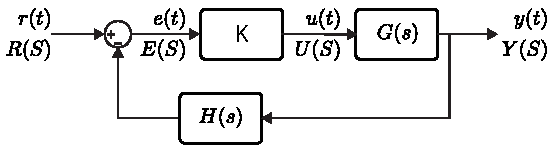
\includegraphics[width=\textwidth]{P}
    \end{center}
\end{minipage}
\end{center}

The closed loop transfer function of this basic control system is
%
\begin{align*}
\frac{Y(s)}{R(s)} = \frac{K G(s)}{1 + K G(s) H(s)} =\frac{K G(s)}{1 + K G_{OL}(s)}
\end{align*}
%
where the poles of the closed loop system are
the roots of the characteristic equation 
%
\begin{align*}
1 + K G_{OL}(s) = 0 
\\
1 + K \frac{n(s)}{d(s)} = 0 
\end{align*}
%
The goal is deriving the qualitative and quantitive behavior of
closed-loop pole ``paths'' for \textbf{positive} gain $K$ that 
solves the equation $1 + K G_{OL}(s) = 0$ (or $1 + K \frac{n(s)}{d(s)} = 0$).

\subsection{Angle and Magnitude Conditions}

Let's analyze the characteristic equation 
%
\begin{align*}
K G_{OL}(s) = -1 \quad , \mathrm{or} \quad K \frac{n(s)}{d(s)} = -1 
\quad , \mathrm{or} \quad 
K \frac{(s - z_1) \cdots (s - z_M)}{(s - p_1) \cdots (s - p_N)} 
&= -1
\end{align*}
%
Let's derive the \textbf{magnitude condition} given that $K > 0$,
%
\begin{align*}
K | G_{OL}(s) | = 1 \quad , \mathrm{or} \quad K  \left| \frac{n(s)}{d(s)} \right| = 1 
\quad , \mathrm{or} \quad 
K \frac{|s - z_1| \cdots |s - z_M|}{|s - p_1| \cdots |s - p_N|}  = 1
\end{align*}
%
Now let's derive the \textbf{angle condition} given that $K > 0$,
%
\begin{align*}
\angle [ G_{OL}(s) ] = \pi (2 k + 1) 
\quad ,  &\mathrm{or} \quad 
\angle [n(s)] - \angle [d(s)] = \pi (2 k + 1) 
\\
\quad , &\mathrm{or} \quad 
\angle [s - z_1] \cdots \angle [s - z_M] - \left( \angle [s - p_1] \cdots \angle [s - p_N] \right)
= \pi (2 k + 1), 
\ \ k \in \mathbb{Z} 
\end{align*}
%
For a given $K$, s values that satisfy both magnitude and angle
conditions are located on the root loci. These constitutes the most
fundamental knowledge regarding the root locus analysis.

How we can check whether a candidate $s^*$ is in the root -locus or not.
If we analyze the angle condition, we can see that it is independent 
from the parameter $K$. However, If we focus on the magnitude condition, 
we can see that 
%
\begin{align*}
K = \frac{1}{| G_{OL}(s^*) |} = \left| \frac{d(s^*)}{d(s^*)} \right| = 
\frac{|s^* - p_1| \cdots |s^* - p_N|}{|s^* - z_1| \cdots |s^* - z_M|} 
\end{align*}
%
which implies that for every $s^*$ candidate (that is not a pole or zero), 
we can indeed compute a gain $K$ value.

In conclusion, only angle condition is used for testing 
whether a point is in the root-locus or not. On the other hand, 
will use the magnitude condition to compute the 
value of gain $K$, if we find that a candidate $s^*$
is in the root locus based on the angle condition.

\newpage

\textbf{Ex:} It is given that $G_{OL}(s) = \frac{1}{s (s+4)}$.
Determine if the following pole candidates are on the 
root-locus or not
%
\begin{align*}
	p_1^* &= -2  \ , \  p_2^* = 2 \,\ p_3^* = -2 + 2 j
\end{align*}
 
 \textbf{Solution:}  We only test the angle
 condition. Solutions are illustrated on the $s-$planes
provided below

 \begin{center}
\begin{minipage}[h]{\linewidth}
    \begin{center}
      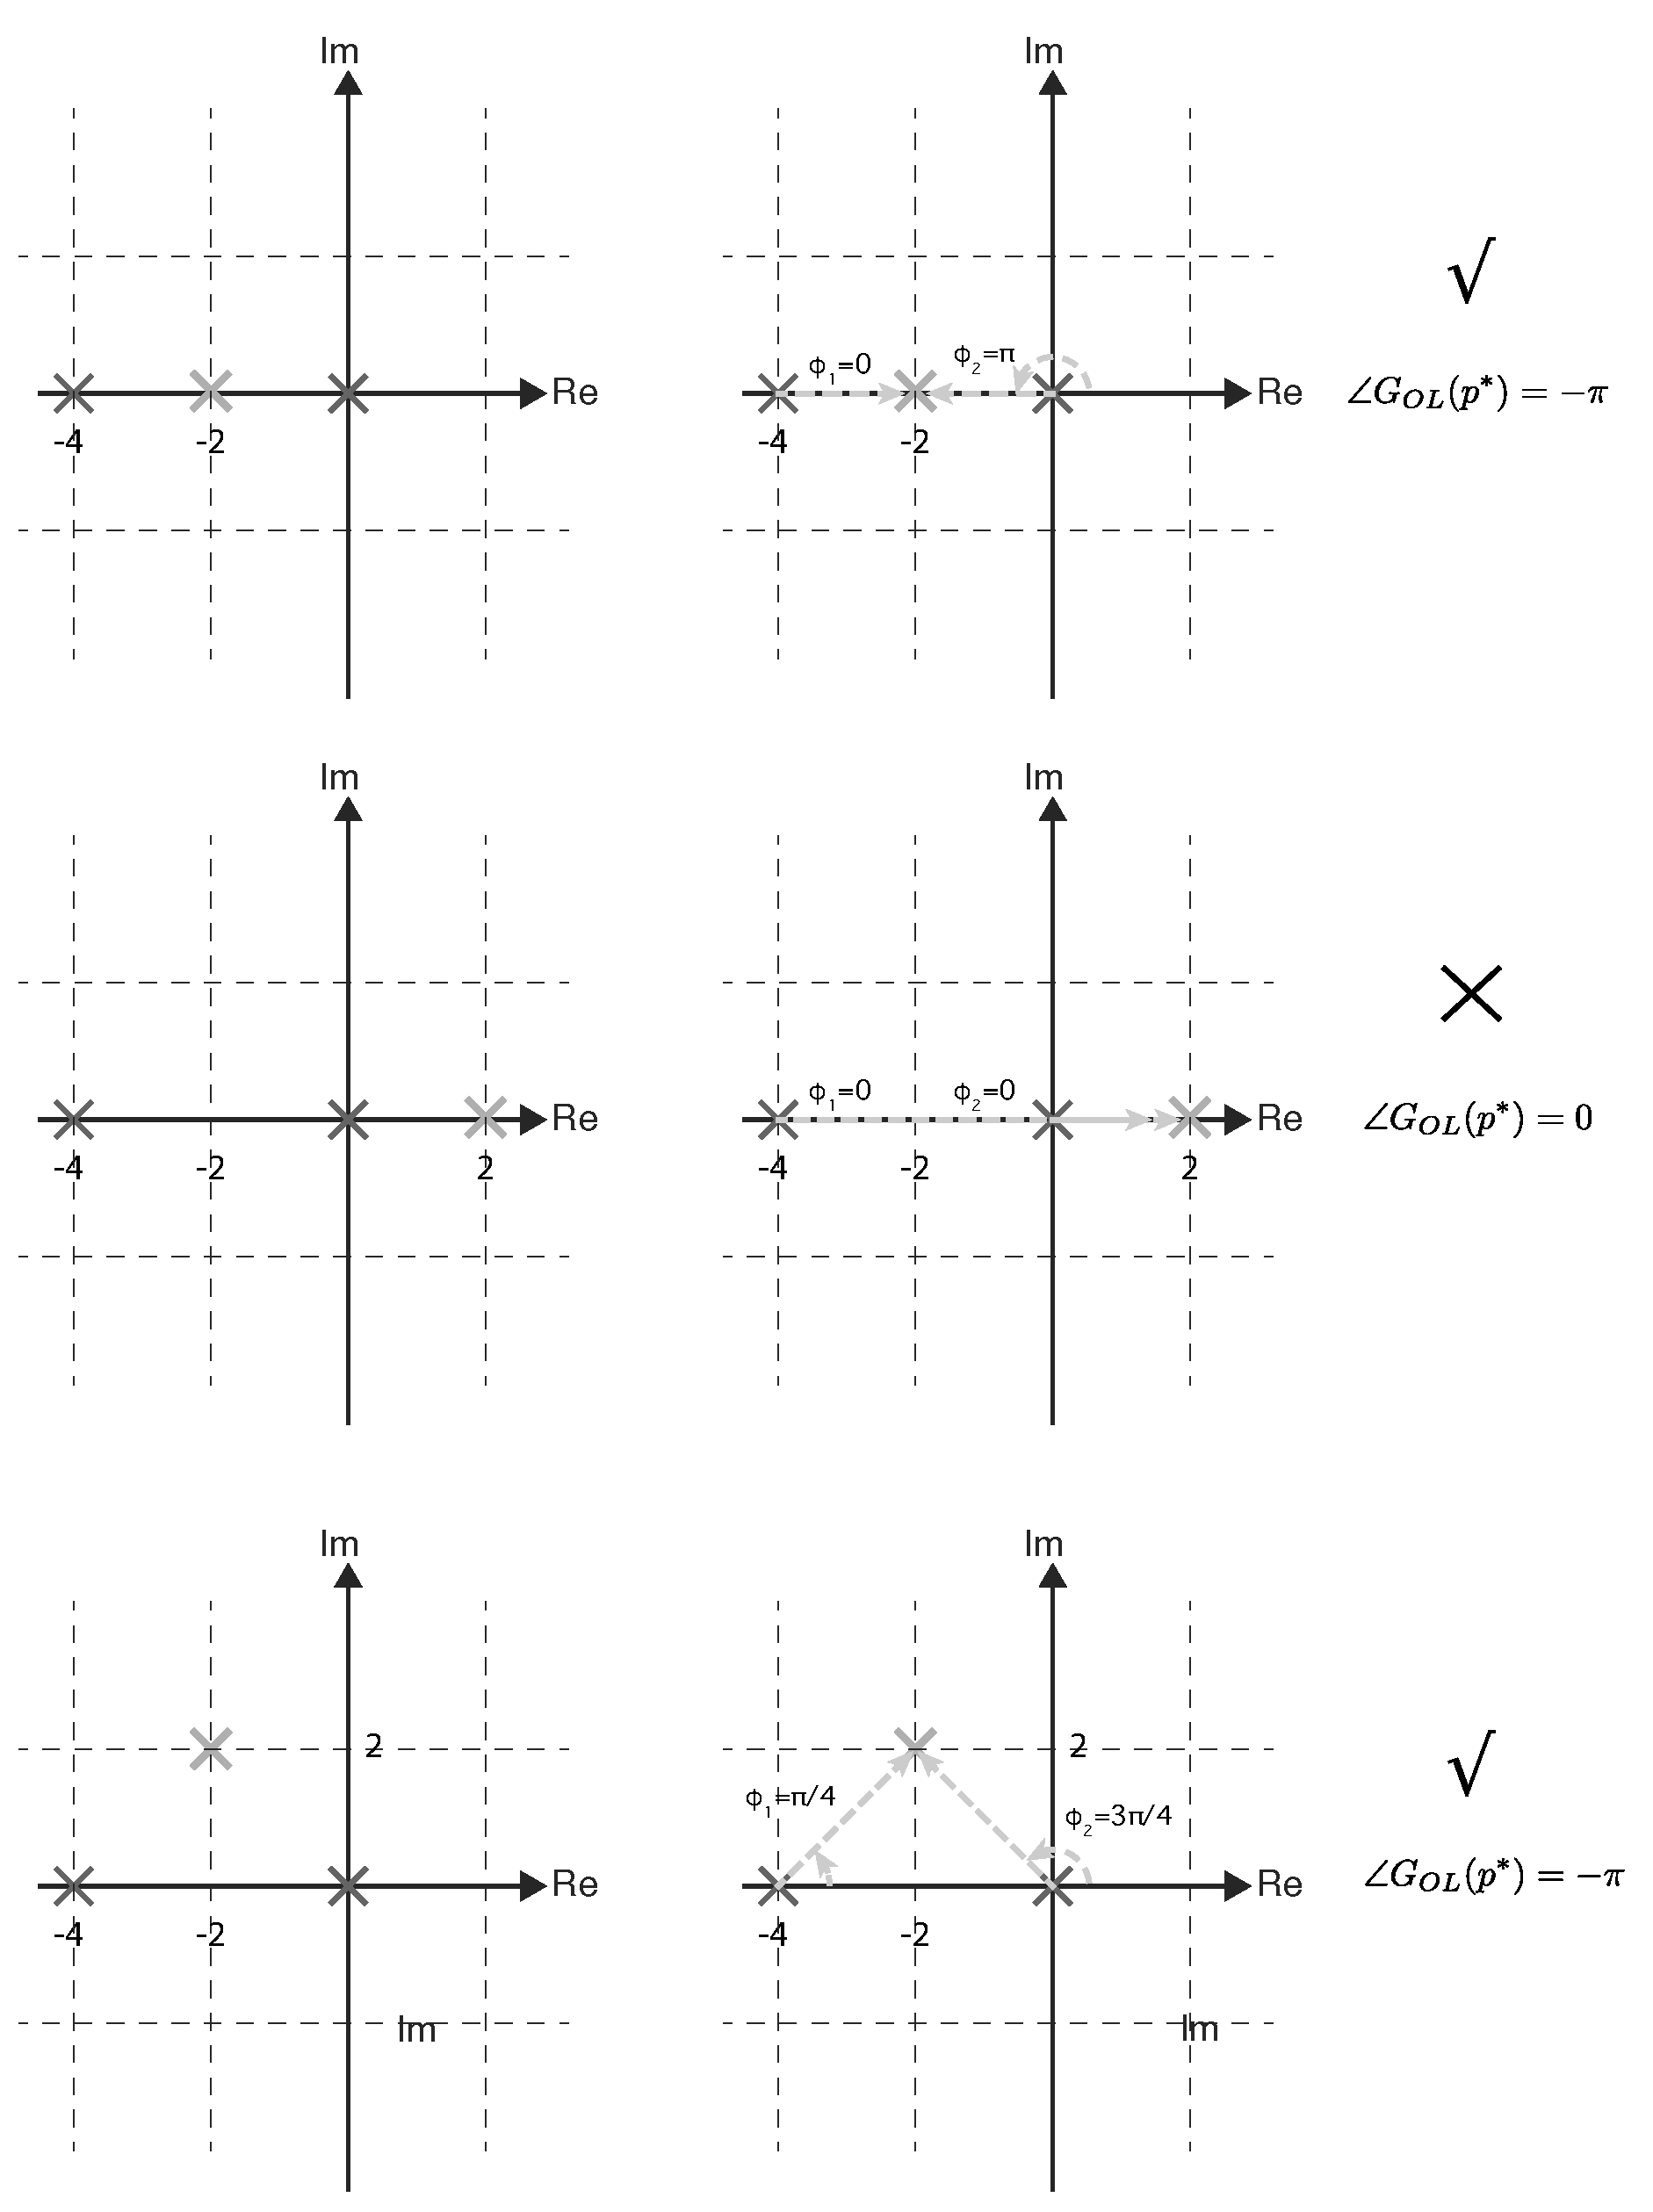
\includegraphics[width=0.85\textwidth]{exangle}
    \end{center}
\end{minipage}
\end{center}

\subsection{Rules and procedure for constructing root loci}

\begin{enumerate} 

\item Compute the zeros poles of the open-loop 
transfer function and write the characteristic eqiation
of closed-loop system.
%
\begin{align*}
1 + K G_{OL}(s)  &= 0 \\
1 + K \frac{n(s)}{d(s)} &= 0 \\
1 + K \frac{(zs- z_1) \cdots (zs- z_M)}{(s - p_1) \cdots (s - p_N)} &= 0 \\
\end{align*}
%

\item Root loci has $N$ separate branches. Since,
%
\begin{align*}
\left[ (s - p_1) \cdots (s - p_N) \right] + K \left[ (zs- z_1) \cdots (zs- z_M) \right]  &= 0 \\
d(s) + K n(s) = 0
\end{align*}
%
has $N$ number of roots for all $K$.

\item Root loci starts from poles of $G_{OL}(s)$ and 
%
\begin{enumerate} 
   \item $M$ branches terminates at the zeros of $G_{OL}(s)$
   \item $N-M$ branches terminates at $\infty$ (implicit zeros of $G_{OL}(s)$)
\end{enumerate}

It is relatively easy to understand this 
%
\begin{align*}
d(s) + K n(s) = 0 
\\
K \to 0 \ \Rightarrow \ [d(s) + K n(s) = 0 \ \to \ [d(s) = 0]
\\
K \to \infty \ \Rightarrow \ [d(s) + K n(s) = 0 \ \to  \ [n(s) = 0]
\end{align*}

\item Root loci on the real axis determined by open-loop zeros and
  poles. $s = \sigma \in \mathbb{R}$ then, based on the angle condition
  we have
%
\begin{align*}
\mathrm{Sign} [ G_{OL}(\sigma) ] &= -1
\end{align*}
%
Let's first analyze the effect of complex conjugate pole/zero (and double pole/zero on real axis)
pairs on the equation above. Let $\sigma^* \in \mathbb{R}$  is the candidate location and complex
conjugate poles has the following form $p_{1,2} = \sigma \pm j \omega$
\begin{align*}
\mathrm{Sign} [ ( \sigma^* + \sigma - j \omega) (\sigma^* + \sigma + j \omega) ] &= \mathrm{Sign} [ (\sigma^* + \sigma)^2 + \omega^2 ] 
= 1 
\end{align*}
%
We can see that complex conjugate zero/pole pairs have not effect 
on angle condition for the roots on the real axis. Then for
the remaining ones we can derive the following condition
%
\begin{align*}
\mathrm{Sign} [ G_{OL}(\sigma) ] = \prod_{i=1}^{\bar{M}}  \mathrm{Sign} [\sigma - z_i]
  \prod_{j=1}^{\bar{N}}  \mathrm{Sign} [\sigma - p_j] = -1
\end{align*}
%
which means that for ODD number of poles $+$  zeros 
$\mathrm{Sign} [\sigma - p_i ]$ and $\mathrm{Sign} [\sigma - z_i] $ 
must be negative for satisfying this condition for that particular $\sigma$
to be on the root-locus. We can summarize the rule as

\textbf{If the test point $\sigma$ on real axis has ODD numbers of 
poles and zeros in its right, then this point is located 
on the root-locus.}

\newpage

\textbf{Ex:} The figure below illustrates the root locus plots
of three different transfer functions.

\begin{center}
\begin{minipage}[h]{0.99\linewidth}
    \begin{center}
      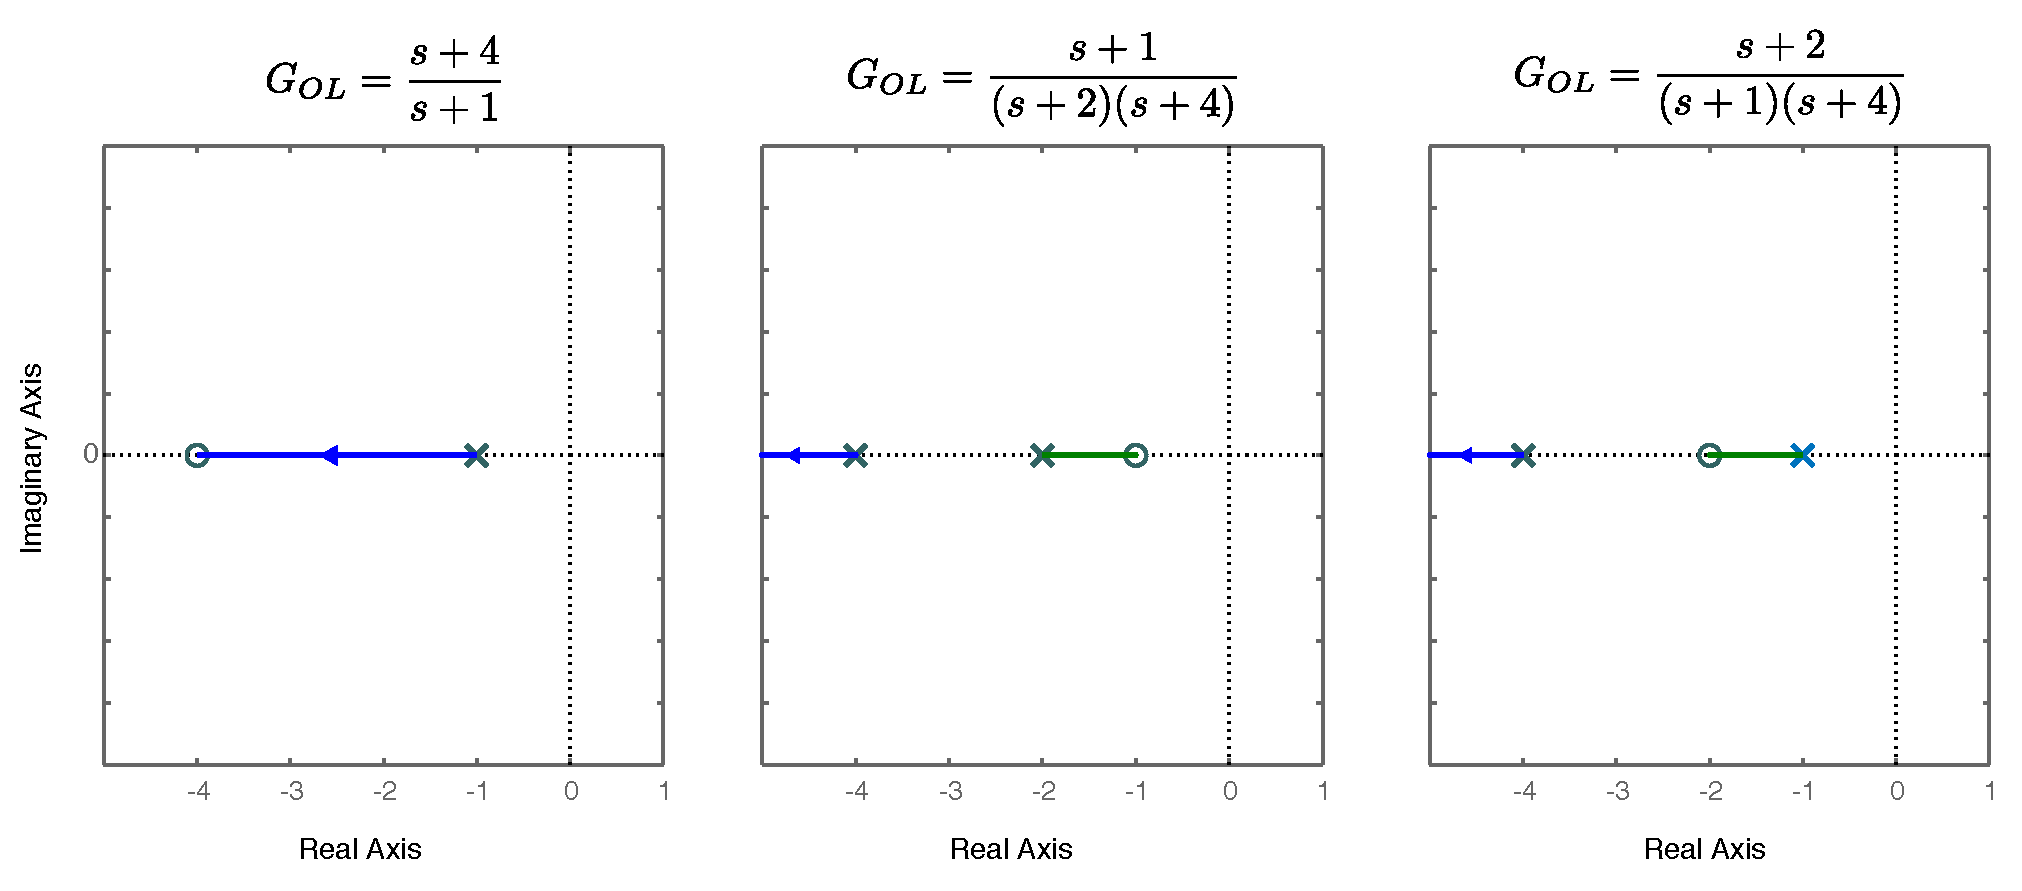
\includegraphics[width=\textwidth]{realaxis}
    \end{center}
\end{minipage}
\end{center}

\item Asymptotes

\begin{itemize}
  \item $N-M$ branches goes to infinity. Thus, there exist $N-M$ many
    asymptotes
  \item For large $s$ we can have the following approximation
 \begin{align*}
  &K \frac{(s - z_1) \cdots (s - z_M)}{(s - p_1) \cdots (s - p_N)}
   \approx \frac{K}{s^{N-M}}
\\
&\angle \left[ \frac{K}{s^{N-M}} \right] = -(N-M) \angle [ s ] = \pi (2 k + 1), \ k \in \mathbb{Z} 
\\
&\phi_{a} = \frac{\pm \pi (2 k + 1)}{N-M}, \ k \in \lbrace 1, \cdots, N-M \rbrace
 \end{align*}
%
  \item Real axis intercept $\sigma_c$ can be computed as
 \begin{align*}
   \sigma_c = \frac{\sum p_i - \sum z_i}{N-M}
 \end{align*}
%
This can be derived via a different approximation (see textbook)
\end{itemize}

\newpage

\textbf{Ex:} The figure below illustrates the root locus plots
of two different transfer functions.

\begin{center}
\begin{minipage}[h]{0.9\linewidth}
    \begin{center}
      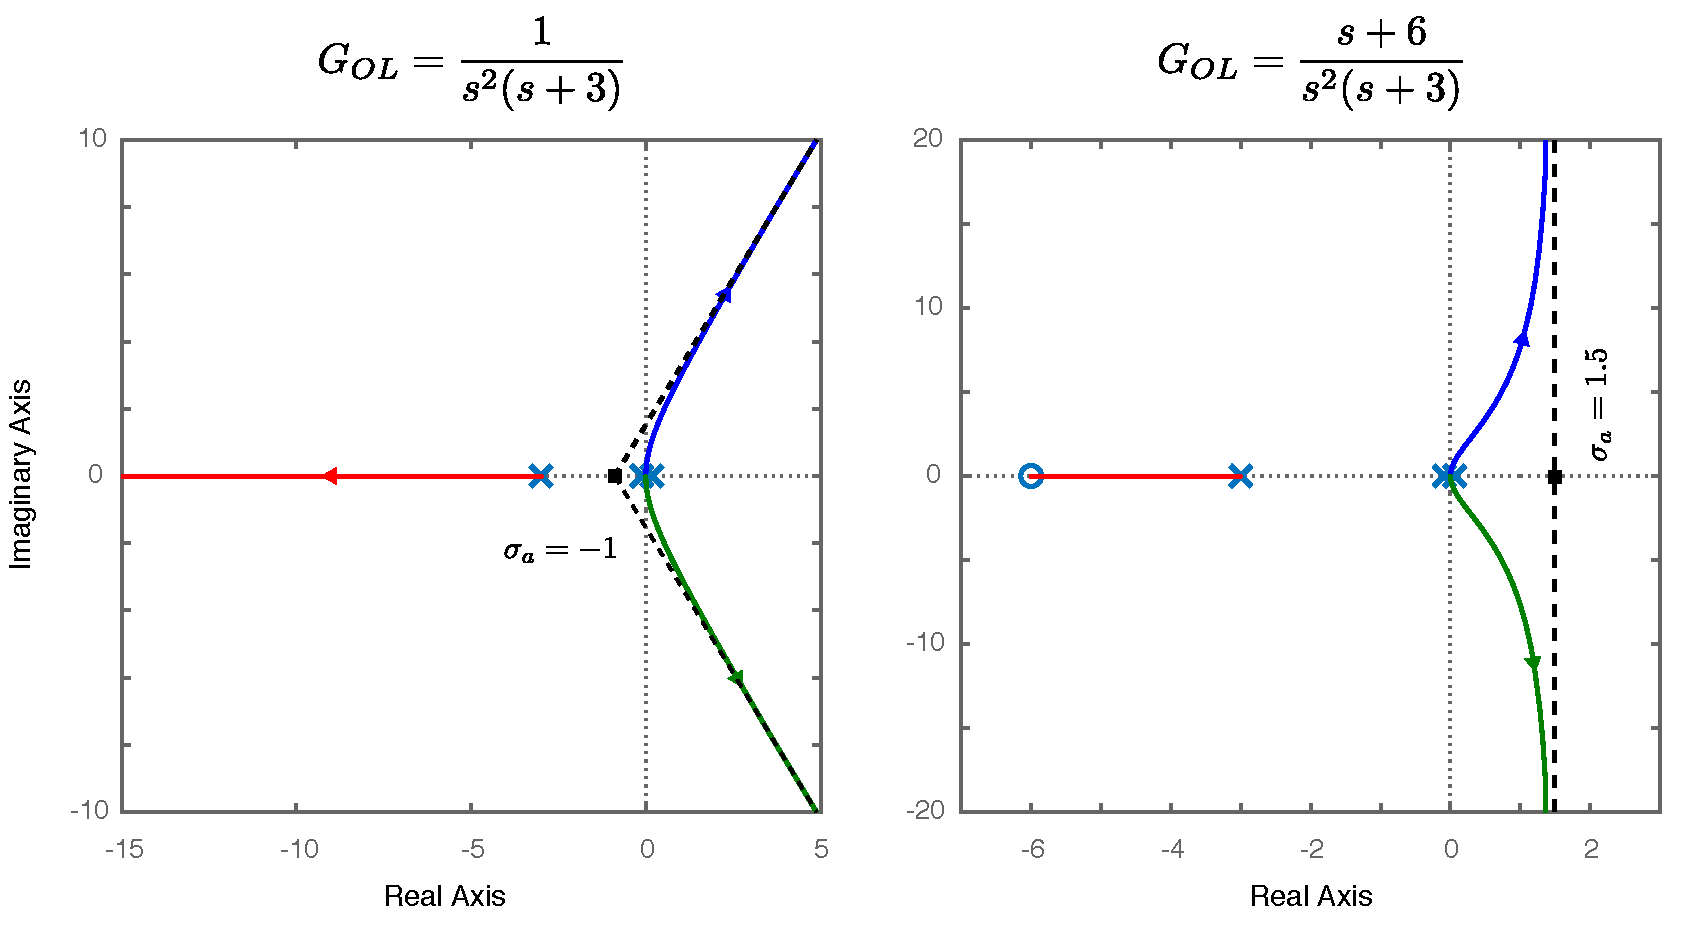
\includegraphics[width=\textwidth]{asm}
    \end{center}
\end{minipage}
\end{center}

\item Breakaway and break-in points on real axis. When s is real 
$s = \sigma, \ \sigma \in \mathbb{R}$, we have
%
\begin{align*}
1 + K G_{OL} (\sigma) &= 0 
\end{align*}
%
Note that break-in and breakaway points corresponds to 
double roots. Thus, if $\sigma_{b}$ is a break-away or break-in 
point we have 
%
\begin{align*}
1 + K G_{OL} (\sigma_b) &= 0 
\\
K \left[ \frac{d}{d \sigma} G_{OL}(\sigma) \right]_{\sigma_b} &= 0
\end{align*}
%
Thus, we conclude that break-in or break-away points satisfy
the following conditions
%
%
\begin{align*}
\left[ \frac{d G_{OL}(\sigma)}{d \sigma} \right]_{\sigma = \sigma_b} = 0
\quad ,
K(\sigma_B) = \frac{-1}{G_{OL} (\sigma_b) }
\quad ,
K(\sigma_b) > 0
\end{align*}

We can derive two corollary conditions for computing $\sigma_b$ as
%
%
\begin{align*}
\left[ \frac{d}{d \sigma} \frac{1}{G_{OL}(\sigma)} \right]_{\sigma = \sigma_b} = 0
\quad or , \quad
\left[ \left( \frac{d}{d \sigma} N(\sigma) \right) D(\sigma)  -
\left( \frac{d}{d \sigma} D(\sigma) \right)  N(\sigma) \right]_{\sigma_b} = 0
\end{align*}

\newpage

\textbf{Ex:} Draw the root locus diagram for $G_{OL}(s) = \frac{1}{s (s+4)}$,
compute the real axis intercept $\sigma_c$ and break away point (with the associated gain value).

\begin{minipage}[h]{0.5\linewidth}
    \begin{center}
      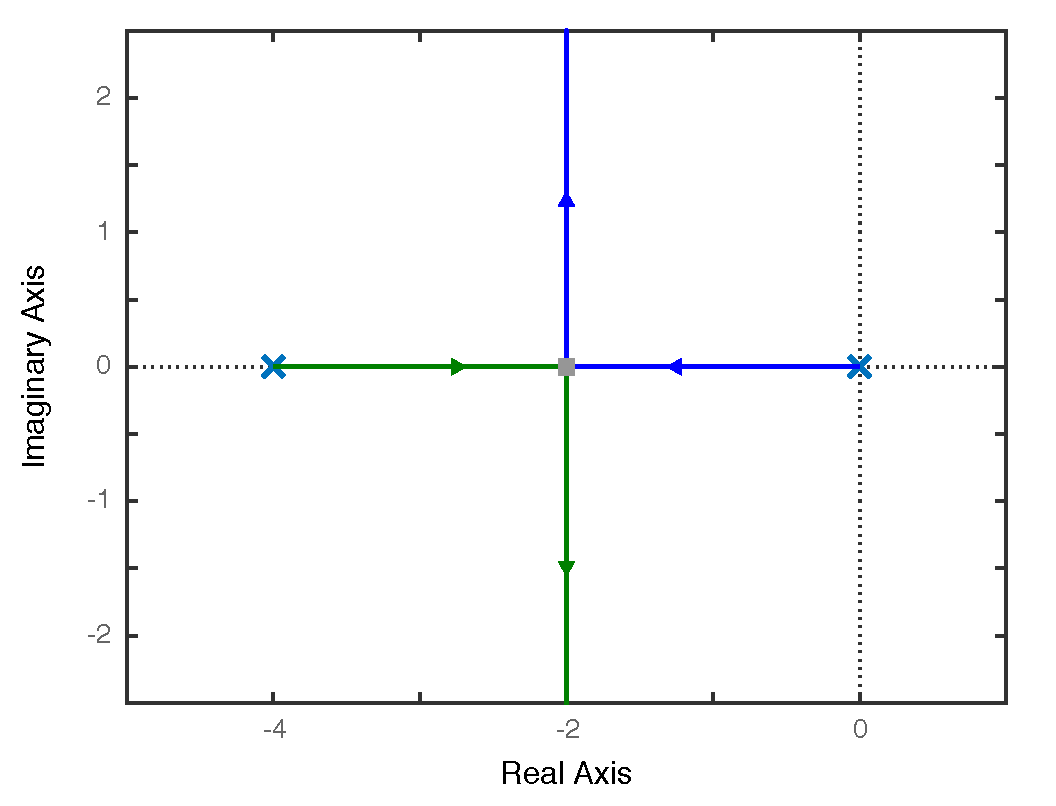
\includegraphics[width=\textwidth]{break_away}
    \end{center}
\end{minipage}
\begin{minipage}[h]{0.5\linewidth}
	\begin{align*}
	\sigma_c &=  -2
	\\
	\sigma_{ba} &=  -2 \quad , \ K(\sigma_{ba}) = 4
	\end{align*}
\end{minipage}

\vspace{12pt}

\textbf{Ex:} Draw the root locus diagram for $G_{OL}(s) = \frac{s+4}{s (s+3)}$,
compute the break-away and break-in points (with the associated gain values).

\begin{minipage}[h]{0.5\linewidth}
    \begin{center}
      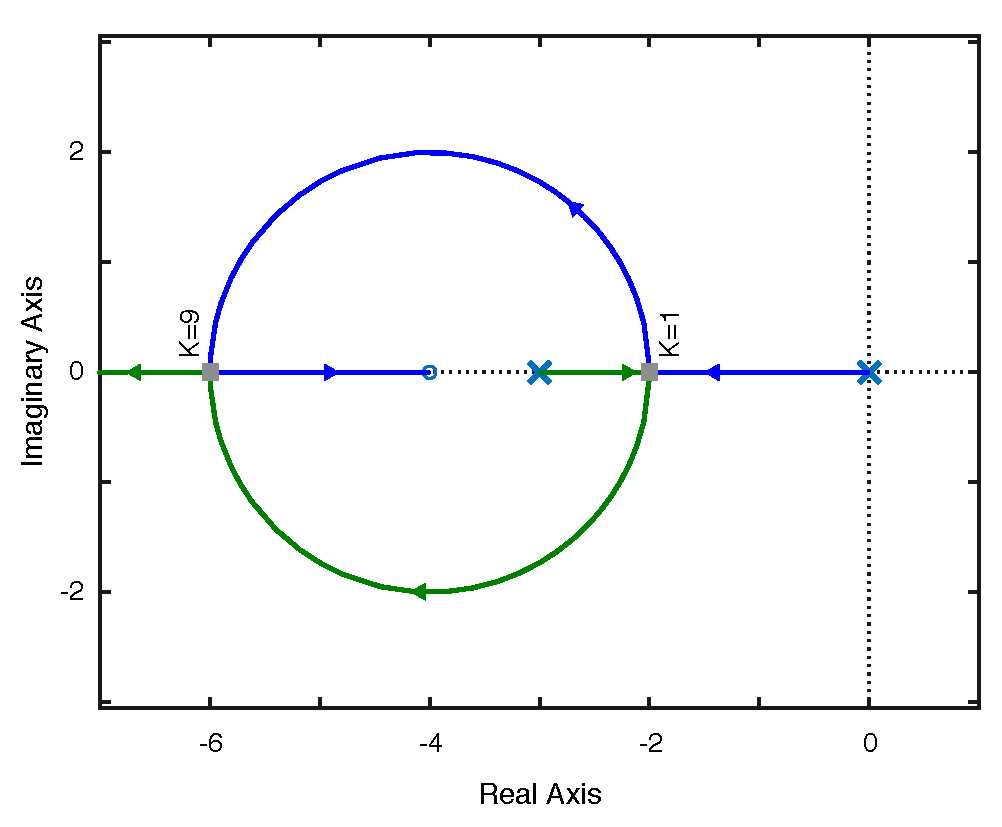
\includegraphics[width=\textwidth]{bin_baway}
    \end{center}
\end{minipage}
\begin{minipage}[h]{0.5\linewidth}
	\begin{align*}
	\sigma_{b}^2 + 8 \sigma_b + 12 = 0 
	\\
	\sigma_{b-a} =  -2 \quad , \ K(\sigma_{b-a}) = 1
	\\
	\sigma_{b-in} =  -6 \quad , \ K(\sigma_{b-in}) = 9
	\end{align*}
\end{minipage}

\vspace{12pt}

\item Finding the imaginary axis crossings. 

These crossings are particularly important, since at these crossings
(generally)   stability changes. At these points the poles become purely
imaginary $p_{1,2} = \pm j \omega$. If we insert this into characteristic 
equation we get
%
\begin{align*}
1 + K G_{OL} (j \omega) &= 0 \\
D(j \omega) + K N(j \omega) &= 0 \\ ,
\\
\mathrm{Re} \lbrace D(j \omega) + K N(j \omega) \rbrace &= 0 \\
\mathrm{Im} \lbrace D(j \omega) + K N(j \omega) \rbrace &= 0 
\end{align*}
%
Note that depending on the order of the system, 
solving the above equation can be 
most computationally very heavy.

\textbf{Second way} of finding the imaginary axis crossing is to
apply the Routh-Hurwitz criteria. Note that at these crossings the 
system becomes unstable. Using this fact, we can first construct a 
Routh table for the closed-loop characteristic equation and then 
derive the $K$ values where a change of stability occurs. After that, we can
use the computed critical $K$ values to derive the pole locations
on the imaginary axis..

\vspace{6pt}

\textbf{Ex:} Draw the root locus diagram for $G_{OL}(s) = \frac{1}{s (s+2) (s+3)}$,
compute the break-away point and imaginary axis crossings 
(with the associated gain values).

\vspace{12pt}

\begin{minipage}[h]{0.55\linewidth}
    \begin{center}
      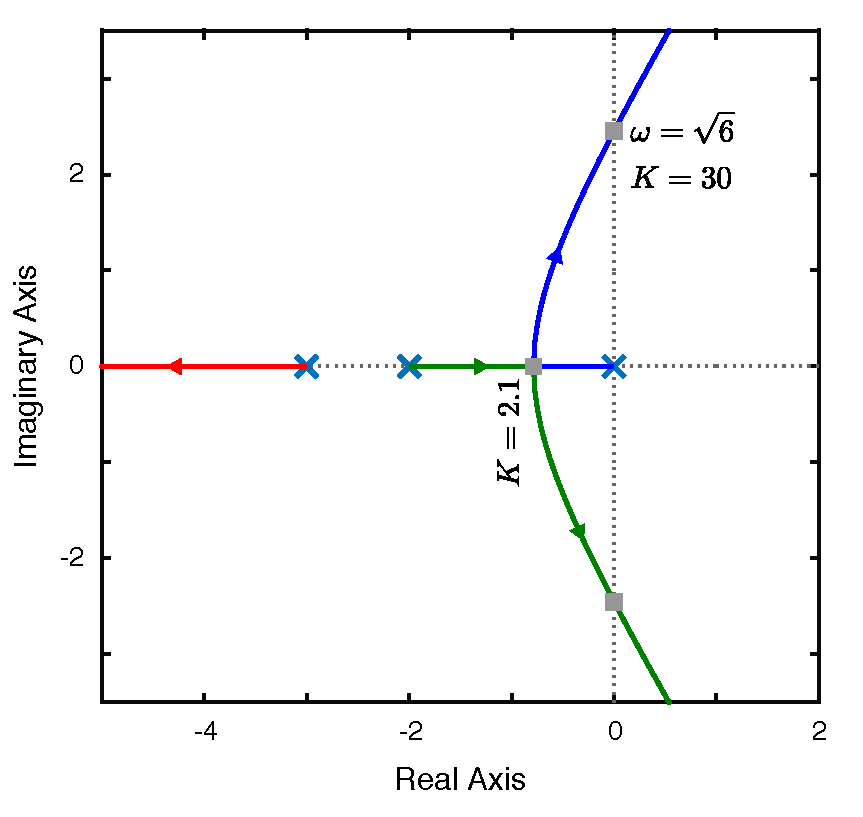
\includegraphics[width=0.95\textwidth]{imag}
    \end{center}
\end{minipage}
\begin{minipage}[h]{0.45\linewidth}
	Break-away point
	\begin{align*}
	& 3 \sigma_{b}^2 + 10 \sigma_b + 6 = 0 
	\\
	& \sigma_{b,1} = - 0.8  \quad , \ K(\sigma_{b,1}) = 2.1 > 0 \rightarrow \mathrm{OK}
	\\
	& \sigma_{b,2} =  -2.5 \quad , \ K(\sigma_{b,2}) = -0.6 < 0 \rightarrow \mathrm{NO}
	\end{align*}
	Imaginary axis crossing
	\begin{align*}
	& D(j \omega) + K (j \omega) = 0 \\ 	 
	& (j \omega)^3 + 5 (j \omega)^2 + 6 (j \omega) + K = 0 \\ 
	& (K - 5 \omega^2) + (6 \omega - \omega^3) j  = 0
	\\ & \Rightarrow \omega = \sqrt{6}  \quad , \ K = 30
	\end{align*}
\end{minipage}

\vspace{12pt}

Now let's find the imaginary axis crossings using the Routh table. 
The characteristic equation for this system is $s^3 + 5 s^2 + 6 s +
K$, then the Routh table takes the form

\vspace{6pt}
\begin{minipage}[h]{1\linewidth}
\begin{center}
\begin{tabular}{|c || c || c | l |}
\hline
$s^3$ & 1 & 6 & 
\\ \hline
$s^2$ & 5 & K & 
\\ \hline
$s^1$ & $\frac{30 - K}{5}$ & 0 & 
\\ \hline
$s^0$ & K & 0 &
\\ \hline
\end{tabular}
\end{center}
\end{minipage}
\vspace{6pt}

We know that in order for the system to stable $K \in (0 , 30)$,
since we only consider positive $K$ values, when $K = 30$
system stability changes (from stable to unstable). Let $K=30$
and re-form the Routh table. 

\vspace{6pt}
\begin{minipage}[h]{1\linewidth}
\begin{center}
\begin{tabular}{|c || c || c | l |}
\hline
$s^3$ & 1 & 6 & 
\\ \hline
$s^2$ & 5 & 30 & $\rightarrow A(s) = 5 s^2 + 30$
\\ \hline
$s^1$ & 10 & 0 &  $\leftarrow A'(s) = 10 s $
\\ \hline
$s^0$ & 30 & 0 &
\\ \hline
\end{tabular}
\end{center}
\end{minipage}
\vspace{6pt}

Based on the Routh table, we conclude that when $K = 30$, system
becomes unstable, the unstable poles are located on the imaginary
axis, and their locations can be find using the Auxiliary polynomial 
as
%
\begin{align*}
A(s) = 0 \rightarrow p_{1,2} = \pm \sqrt{6} j
\end{align*}
%

\newpage

\subsection{Root-locus with respect to different parameters}

Let's consider the following feedback control system. 
We wonder the location of closed-loop
poles with respect to the parameter $A$ which does not directly fit to
the classical form of root-locus. 

\begin{center}
\begin{minipage}[h]{\linewidth}
    \begin{center}
      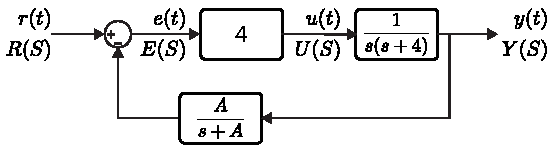
\includegraphics[width=0.5\textwidth]{lowpass}
    \end{center}
\end{minipage}
\end{center}

Let's first compute the closed-loop TF and analyze the characteristic
equation.
%
\begin{align*}
  \frac{Y(s)}{R(s)} &= \frac{ K G(s) }{1 + K G(s) H(s)} 
\\
  &= \frac{ s+A }{s (s+4) (s+A) + 4 A }
\\
 &= \frac{ s+A }{s^3 + (A + 4) s^2 + 4 A s + 4 A}
\end{align*}
%
Now let's organize the characteristic equation
%
\begin{align*}
(s^3 + 4 s^2) + A  (s^2 + 4 s + 4) = 0
\end{align*}
%
If we divide the characteristic equation by $(s^3 + 4 s^2)$ we obtain
%
\begin{align*}
1+ A \frac{s^2 + 4 s + 4}{s^3 + 4 s^2} &= 0
\\
1+ A \bar{G}_{OL}(s) &= 0
\end{align*}
%
Now if we consider $\bar{G}_{OL}(s)$ as the open-loop transfer
function and draw the root-locus, 
then we would derive the dependence 
of the roots to the parameter A. 

Root-locus of the system w.r.t parameter $A > 0$ is given below.

\begin{center}
\begin{minipage}[h]{\linewidth}
    \begin{center}
      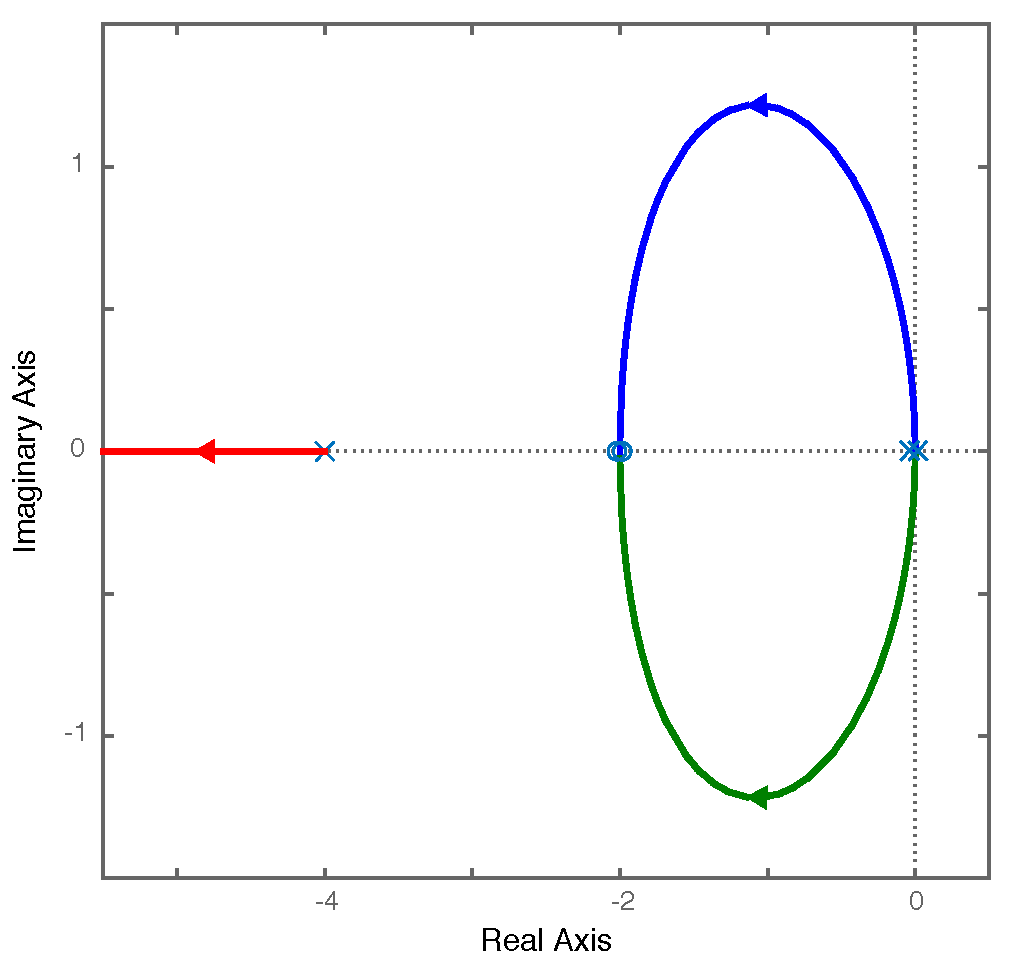
\includegraphics[width=0.5\textwidth]{rlocusA}
    \end{center}
\end{minipage}
\end{center}

\end{enumerate}

% **** This ENDS THE EXAMPLES. DON'T DELETE THE FOLLOWING LINE:
\end{document}